\documentclass[10pt]{article} 
\usepackage{simpleConference}
\usepackage[utf8]{inputenc} %unicode support
\usepackage{parskip}
\usepackage[hidelinks]{hyperref}
\usepackage{tcolorbox}
\usepackage{pdfpages}
\newcommand*{\quedb}{\hfill\ensuremath{\square}}%
\usepackage{anyfontsize}
\usepackage{linguex}
\usepackage{mathtools}
%\usepackage[applemac]{inputenc} %applemac support if unicode package fails
%\usepackage[latin1]{inputenc} %UNIX support if unicode package fails
%\DeclarePairedDelimiter\abs{\lvert}{\rvert}%
%\DeclarePairedDelimiter\norm{\lVert}{\rVert}%

\usepackage{times}
\usepackage{graphicx}
\usepackage{amssymb}

% additional packages
\usepackage{amsmath}
\usepackage{bbm}
\usepackage{support-caption}
\usepackage{subcaption}
\usepackage{tikz, tikz-3dplot} 
\usetikzlibrary{calc}
\usetikzlibrary{matrix}
\usepackage{url}
%\usepackage{hyperref}
\usepackage{float}
\usepackage{amsthm}
\usepackage{booktabs}

%\startlocaldefs
% macros
\newtheorem{theorem}{Theorem}
\newtheorem{lemma}[theorem]{Lemma}
\newtheorem{proposition}[theorem]{Proposition}
\newcommand{\norm}[1]{\left\lVert#1\right\rVert}
\providecommand{\keywords}[1]{\textbf{\textit{Keywords:}} #1}
%\endlocaldefs

\begin{document}

\title{On Storey's direct approach to false discovery rates}
\author{Marko Lalović
\\
July 2019 \\
}

\maketitle

\begin{abstract}
Storey~\cite{Storey} shed a new light on multiple-testing problem with the definition of positive false discovery rate measure and gave new perspective with direct approach to false discovery rates.

We provide formal introduction to multiple-testing problem and intuitive explanation of Storey's direct approach. We demonstrate the duality between Storey's direct approach and Benjamini-Hochberg (BH) procedure~\cite{BH} when using Storey's estimate $\widehat{\pi}_{0}$ of the proportion of null hypotheses $\pi_{0}$ in BH procedure. 

We show that the estimator $\widehat{\pi}_{0}$ of the proportion of null hypotheses $\pi_{0}$ plays a key role in multiple-testing problem and that the approach we take doesn't matter much. We confirm this using simulations where performances were practically identical for both methods.

We show that Storey's estimator $\widehat{\pi}_{0}$ can be very upward biased when distance between distributions under null hypothesis and alternative hypotheses is small. In our simulations this upward bias of $\widehat{\pi}_{0}$ was reduced if we increased the value of the tuning parameter $\lambda$ and especially by tuning this $\lambda$ parameter using the bootstrap method. However this bootstrap method can result in underestimation of $\pi_{0}$, as already explained in~\cite{Black}. 

In case of dependence Storey suggested the same approach~\cite{Dependence}. We show, this time only using simulation, that dependence can lead to a very high overestimation of false discovery rate.
\end{abstract}

\keywords{Multiple testing, Multiple comparisons, False discovery rate}

\tableofcontents
%\newpage

%  on the basis of some test statistic $P$. usually about the population parameter based on a sample
\section{Introduction} \label{sec: intro}

\subsection{Single-hypothesis testing}
Following the scientific method, researchers normally want to establish the truth of a statement by showing that the opposite appears to be false. In general, a {\it hypothesis} is a proposed explanation for a phenomenon that one can test. In statistics, the hypotheses involve a parameter $\theta$ whose value is unknown but must lie in a certain parameter space $\Omega$. We assume that $\Omega$ can be partitioned into two disjoint subsets $\Omega_0$ and $\Omega_1$ and define two hypotheses:
\begin{align*}
H_{0}\text{: } \theta &\in \Omega_0, \\
H_{1}\text{: } \theta &\in \Omega_1.
\end{align*}

The hypothesis $H_{1}$ is the statement that confirms the theory and it is called an {\it alternative hypothesis}. The opposite $H_{0}$ is called a {\it null hypothesis}. We must decide which of the hypotheses appears to be true. A procedure for deciding this is called a {\it test procedure} or simply a {\it test}. Before we have to decide which hypothesis to choose, we assume that we can observe a random sample $\mathbf{X} = (X_{1}, ..., X_{n})$ drawn from a distribution that involves the unknown parameter $\theta$. Let $T = r(\mathbf{X})$ be a statistic and let $\Gamma$ be a subset of the real line and suppose that the test procedure is of the form: reject $H_{0}$ if $T \in \Gamma$. Then $T$ is called a {\it test statistic} and $\Gamma$ a {\it rejection region}. A problem of this type is called a {\it single-hypothesis testing}.

In single-hypothesis testing we only have two kinds of errors we might make. A {\it type I error} occurs when we reject the null $H_{0}$ when in fact $H_{0}$ is true. A {\it type II error} occurs when we fail to reject the null $H_{0}$ when in fact $H_{0}$ is false. The {\it significance level $\alpha$} is the upper bound on the probability of type I error:
\begin{equation} \label{eq: condition1}
	\text{Pr}(T \in \Gamma \mid H_{0} \text{ is in fact true }) \leq \alpha.
\end{equation}

The {\it detection power $\pi$} of a test is the probability of rejecting $H_{0}$ when in fact $H_{0}$ is false. Statistical practice is to choose the value of $\alpha$, say $0.01$, and then find the rejection region $\Gamma_{\alpha}$ that maximizes the detection power and satisfies Eq.~\ref{eq: condition1}, that probability of type I error is at most $\alpha$. The detection power $\pi$ is a function of rejection region $\Gamma_{\alpha}$:
\begin{equation}
	\pi(\Gamma_{\alpha}) = \text{Pr}(T \in \Gamma_{\alpha} \mid H_{0} \text{ is in fact false }).
\end{equation}

Typically, rejection regions $\Gamma_{\alpha}$ and $\Gamma_{\alpha'}$ for different values $\alpha$ and $\alpha'$, are nested in this sense:
\begin{equation} \label{eq: nesting}
	\text{if} \quad \alpha < \alpha' \quad \text{then} \quad \Gamma_{\alpha} \subset \Gamma_{\alpha'}.
\end{equation}

% p-value as a function p: sample space --> (0, 1)
% such that p(x) = inf{alpha: reject at level alpha}
% Pr(p(x) leq alpha) leq alpha

For the given observation $T = t$, the smallest significance level $\alpha$ at which a null hypothesis would be rejected, is called the {\it $p$-value}:
\begin{equation}
	p(t) = \inf \lbrace \alpha : t \in \Gamma_{\alpha} \rbrace.
\end{equation}


\subsection{Multiple-hypothesis testing}
Now consider simultaneous testing a collection of $m$ hypotheses, called a {\it family of hypotheses $\mathcal{F}$}, where for $i = 1, ..., m$, we test $H_{0i}$ versus $H_{1i}$ on the basis of test statistics given in the form of p-values $p_{i}$. Let $H_{1}, ...,H_{m}$ be random variables, where 
\[
	H_{i} = \begin{cases}
		0 & \text{if $H_{0i}$ is in fact true,}\\
		1 & \text{if $H_{1i}$ is in fact true.}
	\end{cases}
\]

A {\it multiple-testing procedure} is a decision function $\phi$, which for a given p-values $p_{1}, ..., p_{m}$ assigns decision values $D_{1}, ..., D_{m}$: 
\begin{equation}
\phi(p_{i}) = D_{i}, \quad i = 1,..., m,
\end{equation}
where $D_{i} = 1$ if hypothesis $H_{0i}$ is rejected and $D_{i} = 0$ otherwise, for each $i = 1,..., m$. Table~\ref{tab: summary} describes the possible outcomes from $m$ hypothesis tests, where $I_{0} \subset \lbrace 1, ..., m \rbrace$ is the index of true null hypotheses, $m_{0} = |I_{0}|$ is the number of true null hypotheses, $V = \sum_{i=1}^{m} (1 - H_{i}) D_{i}$ is the number of true null hypotheses which are rejected (type I errors), $R = \sum_{i=1}^{m} D_{i}$ is the number of all rejected null hypotheses, etc. 

\begin{table}[ht!]
	\centering
	\begin{tabular}{c c c c}
		\hline\hline
		& Accepted     & Rejected & Total \\ [0.5ex]
		\hline
		$I_{0}$ & $U$  & $V$ & $m_{0}$ \\
		$\lbrace 1, ..., m \rbrace \setminus I_{0}$ & $T$  & $S$ & $m - m_{0}$ \\
		Total         & $W$  & $R$ & $m$
	\end{tabular}
	\caption{All possible outcomes from $m$ hypothesis tests.}
	\label{tab: summary}	
\end{table}


If the decision function $\phi$ is based on rejection region of the form $[0, \gamma]$ for some threshold $\gamma > 0$:
\begin{equation}
	\phi(p_{i}) = \mathbbm{1} (p_{i} \leq \gamma),
\end{equation}
then the random variables $U, V, ..., R$ depend only on this threshold $\gamma$, e.g.\ $R(\gamma) = \sum_{i=1}^{m}{\mathbbm{1}{(p_{i} \leq \gamma)}}$.

Good scientific practice requires the specification of certain type I error measure control to be done prior to the data analysis. The problem is to find a multiple-testing procedure which maximizes detection power and satisfies certain conditions involving type I error measures. A problem of this type is called a {\it multiple-testing problem}. It is described in~\cite{RHeller} or in the context of assessing the feature significance in~\cite{ESL}. 

We say that some multiple-testing procedure $\phi$ has {\it strong level $\alpha$ control} of some error measure EM, if it satisfies the condition:
\begin{equation}
\text{EM}_{\phi} \leq \alpha
\end{equation}
for any configuration of true and false hypotheses in the family of $m$ hypotheses $\mathcal{F}$.

The first type I error measure that was suggested is the {\it family-wise error rate (FWER)}. This is the probability that we make at least one type I error among the family $\mathcal{F}$ of $m$ hypotheses using some multiple-testing procedure $\phi$:

\begin{equation}
	\text{FWER}_{\phi} = \text{Pr}(V \geq 1).
\end{equation}


\subsection{Multiple-testing procedures}


\subsubsection{Bonferroni correction}

Simple multiple-testing procedure is the Bonferroni correction with the following decision function $\phi$. Reject $H_{0i}$, if $p_{i} \leq \alpha/ m$: 
\begin{equation}
	\phi(p_{i}) = \mathbbm{1}{(p_{i} \leq \frac{\alpha}{m})}.
\end{equation} 

\begin{proposition} \label{prop: Bonf}
	Bonferroni correction ensures strong level $\alpha$ control of FWER:
\end{proposition}
\begin{proof}
	\begin{equation} \label{eq: bonf_control}
	\text{FWER}_{\text{Bonf.}} = \text{Pr}(\bigcup_{i \in I_{0}} \lbrace p_{i} \leq \frac{\alpha}{m} \rbrace) \leq \sum_{i \in I_{0}} \text{Pr}(p_{i} \leq \frac{\alpha}{m})
	= m_{0} \cdot \frac{\alpha}{m} \leq \alpha.
	\end{equation}
\end{proof}

This control comes with no distributional assumptions (e.g. independence) on the test statistics (p-values) or assumptions on the proportion of null hypotheses $m_{0}/m$. Unfortunately, Bonferroni correction has very little detection power when $m$ is large. 

Now we can try to improve detection power of this simple multiple-testing procedure by constructing an estimator $\widehat{m}_{0}$ of the number of true null hypotheses and simply replace $m$ in decision function $\phi$ with the estimator $\widehat{m}_{0}$ to get a new decision function $\phi'$: 
\begin{equation}
	\phi'(p_{i}) = \mathbbm{1}{(p_{i} \leq \frac{\alpha}{\widehat{m_{0}}})}.
\end{equation}

If $\widehat{m}_{0} < m$, we can achieve improvement in detection power using $\phi'$ instead of $\phi$, because the set of hypotheses rejected by $\phi$ are contained in the set of hypotheses rejected by $\phi'$. 

\begin{proposition}
	If the estimator $\widehat{m}_0$ tends to at most overestimate $m_{0}$:
	\begin{equation}
	\text{E}(\widehat{m}_{0}) \geq m_{0},
	\end{equation}
	then improved Bonferroni correction $\phi'$ satisfies strong level $\alpha$ control:
	\begin{equation}
	\text{FWER}_{\phi'} \leq \alpha.
	\end{equation}
\end{proposition}
\begin{proof}
	Simply replace $m$ with $\widehat{m}_{0}$ in the proof of Proposition~\ref{prop: Bonf}:
	\begin{equation}
	\text{FWER}_{\phi'} \leq \frac{m_{0}}{\widehat{m}_{0}} \cdot \alpha.
	\end{equation}
	Take expected value on both sides and use monotonicity of expected value and the fact that expected value of FWER is FWER:
	\begin{equation}
	\text{FWER}_{\phi'} \leq \frac{m_{0}}{ \text{E}(\widehat{m}_{0}) } \cdot \alpha.
	\end{equation}
	Use $\text{E}(\widehat{m}_{0}) \geq m_{0}$:
	\begin{equation}
	\text{FWER}_{\phi'} \leq \frac{m_{0}}{ \text{E}(\widehat{m}_{0}) } \cdot \alpha \leq \alpha.
	\end{equation}	
\end{proof}

From this example of using FWER error measure and Bonferroni multiple-testing procedure we see, that improvement in detection power and control of type I error measure depends on the properties of an estimator $\widehat{m}_{0}$ of $m_{0}$ (or equivalently $\widehat{\pi}_{0}$ of the proportion $\pi_{0} = m_{0}/m$) of the number of true null hypotheses in the family $\mathcal{F}$. More precisely, lower expected value of estimator $\widehat{m}_{0}$ ($\widehat{\pi}_{0}$) leads to a greater detection power, but it also affects type I error measure. 


\subsubsection{Benjamini-Hochberg procedure}

Another way to improve the detection power is by using a more appropriate type I error measure. Benjamini and Hochberg~\cite{BH} introduced a new type I error measure called {\it false discovery rate (FDR)}. This is the expected proportion of false positive results among all the rejected hypotheses when using some multiple-testing procedure $\phi$:

\begin{equation}
\text{FDR}_{\phi} = \text{E}\left(\frac{V}{R} \mid R > 0 \right) \cdot \text{Pr}(R > 0).
\end{equation}

\begin{proposition}
	For any multiple-testing procedure $\phi$: 
	\begin{equation}
		\text{FDR}_{\phi} \leq \text{FWER}_{\phi}
	\end{equation}
	with equality if all null hypotheses in $\mathcal{F}$ are true.
\end{proposition}
\begin{proof}
	\begin{equation}
	\text{FDR}_{\phi} = \text{E}\left[ \frac{V}{R} \cdot \mathbbm{1}{(R > 0)} \right] 
	\leq \text{E}\left[ \mathbbm{1}{(V \geq 1)} \right] = \text{FWER}_{\phi}.
	\end{equation}
	When all null hypotheses in $\mathcal{F}$ are true, $V = R$ and $\text{FDR}_{\phi} = \text{FWER}_{\phi}.$
\end{proof}
Therefore we might achieve improvement in detection power by controlling FDR error measure instead of FWER error measure.

The following multiple-testing procedure is called {\it Benjamini-Hochberg (BH) procedure}. For given level $\alpha$, given ordered, observed p-values $p_{(1)}, ..., p_{(m)}$, calculate:
\begin{equation}
	\widehat{k} = \text{max} \lbrace k : p_{(k)} \leq \alpha \cdot k/m \rbrace,
\end{equation}
and reject all null hypotheses corresponding to $p_{(i)}$ for $i \leq \widehat{k}$. 

For this procedure Benjamini and Hochberg~\cite{BH} showed the following. If test statistics (in our case $p$-values) are independent and in some cases of dependence, regardless of the distribution of the test statistics (in our case distribution of $p$-values) when $H_{0}$ is false, this procedure has a strong level $\alpha$ control of FDR. Moreover it satisfies the property:
\begin{equation}
\text{FDR}_{\text{BH}} \leq \pi_{0} \cdot \alpha \leq \alpha,
\end{equation}
where $\pi_{0}$ is the proportion of true null hypotheses:
\begin{equation}
\pi_{0} = \frac{m_{0}}{m}.
\end{equation}


\subsubsection{Storey's approach}

Storey suggested~\cite{Storey} a modified version of FDR error measure called the {\it positive false discovery rate (pFDR)}:
\begin{equation}
\text{pFDR}_{\phi} = \text{E}\left( \frac{V}{R} \mid R > 0 \right),
\end{equation}
when using some multiple-testing procedure $\phi$. It holds pFDR $\leq$ FDR:
\begin{equation}
	\text{pFDR}_{\phi} \leq \text{pFDR}_{\phi} \cdot \text{Pr}(R > 0) = \text{FDR}_{\phi},
\end{equation} 
because $\text{Pr}(R > 0) \leq 1$. Therefore we might achieve improvement in detection power by controlling error measure pFDR instead of FDR. In case when $\text{Pr}(R > 0)$ is much less than 1, FDR error measure might be misleading and Storey's pFDR error measure is more appropriate. pFDR error measure also has a clean Bayesian interpretation, which we show in Chapter~\ref{sec: estimates} and it is described in~\cite{Bayesian}. 

Storey suggested in~\cite{Storey} a more direct approach to multiple-testing problem. Rather than fixing level $\alpha$ control of some error measure and then estimating the rejection region ($\hat{k}$ in BH procedure) satisfying level $\alpha$ control ($\text{FDR} \leq \alpha$ for BH procedure), we instead fix the rejection region and then estimate some error measure, preferably pFDR.

Important part of Storey's direct approach is Storey's method of estimating the proportion of true null hypotheses $\pi_{0} = m_{0} / m$. For a good estimator of (p)FDR, we require a good estimator of $\pi_{0}$. This problem of estimating $\pi_{0}$ is described in~\cite{Proportion1} and~\cite{Proportion2}. Storey's method of estimating $\pi_{0}$ is based on the following idea. Since the $m$ observed p-values contain information about the proportion of true null hypotheses $\pi_{0}$, Storey introduces a tuning parameter $\lambda \in (0, 1)$ and use information in 
\begin{equation}
	\frac{\# \lbrace p_{i} > \lambda \rbrace}{m}
\end{equation}
to estimate $\pi_{0}$. 

In cases where $m_{0} << m$ (or equivalently $\pi_{0} << 1$), direct approach using Storey's estimators has much more detection power than BH procedure, which takes $m$ instead of an estimate of $m_{0}$. Equivalently, we can improve detection power of BH procedure by using an estimate of $m_{0}$, but it is no longer guaranteed to achieve FDR control at the desired level. One advantage of using direct approach instead of BH procedure is that we can estimate pFDR instead of FDR. 


\subsection{Overview}
After the formal derivation of Storey's estimators for direct approach in Section~\ref{sec: estimates}, we present results in Sections~\ref{sec: 1st} and~\ref{sec: 2nd} of detection power comparison of BH procedure and direct approach using Storey's estimators. We formally justify and generalize this results. In Section~\ref{sec: properties} we show that Storey's estimator $\widehat{\pi}_{0}$ can be very upward biased when distance between distributions under $H_{0}$ and $H_{1}$ is small. It follows from Section~\ref{sec: estimates} that the same bias is present in the estimation of type I error measure. Lastly in Section~\ref{sec: dependence}, we show with simulation that dependence can lead to very high overestimation of FDR. 


\section{Derivation of Storey's estimators for direct approach} \label{sec: estimates}

Direct multiple-testing procedure using Storey's estimates is based on the following Theorem~\ref{thm: pFDR} which is valid under the following assumptions and the assumption that rejection region $\Gamma_{\alpha}$ satisfies the nesting property Eq.~\ref{eq: nesting}. Consider simultaneous testing of $m$ null hypotheses, where for $i = 1, ..., m$, we test $H_{0i}$ versus $H_{1i}$ on the basis of test statistics $p_{i}$, given in the form of p-values and where significance region is $[0, \gamma]$, for a given threshold $\gamma > 0$. Assume $H_{i} \stackrel{iid}{\sim} \text{Bernoulli}(1 - \pi_{0})$, where $H_{i} = 0$ when $H_{0i}$ is in fact true and $H_{i} = 1$ when $H_{0i}$ is in fact false. Assume $p_{i}$ is uniformly distributed on $[0,1]$ when $H_{0i}$ is in fact true. 
	
Denote the density of $p_{i}$, when $H_{0i}$ is in fact false, with $h(p)$ for $p \in [0, 1]$. 

Moreover, the p-values $p_{i}$ are iid continuous random variables $P$ with density:
\begin{equation}
f(p) = \pi_{0} + (1 - \pi_{0}) \cdot h(p), \qquad p \in [0,1].
\end{equation}

\begin{theorem} \label{thm: pFDR}
The posterior probability for a given implicit prior probability $\pi_{0}$ is:
	\begin{equation}
	\text{pFDR}(\gamma) = \text{Pr}(H = 0 \mid P \leq \gamma).
	\end{equation}
\end{theorem}

\begin{proof}
	\begin{align}
	\text{pFDR}(\gamma) 
	&= \text{E} \left[ \frac{V(\gamma)}{R(\gamma)} \mid R(\gamma) > 0 \right] \\
	&= \sum_{k = 1}^{m} \text{E} \left[ \frac{V(\gamma)}{R(\gamma)} \mid R(\gamma) = k \right] \cdot	\text{Pr}(R(\gamma) = k \mid R(\gamma) > 0) \\
	&=  \sum_{k = 1}^{m} \frac{1}{k} \cdot \text{E} \left[ V(\gamma) \mid R(\gamma) = k \right] \cdot	\text{Pr}(R(\gamma) = k \mid R(\gamma) > 0) \label{eq: pFDR}
	\end{align}
	Given $R(\gamma) = k$ and assumption of independent p-values, it follows that $V(\gamma)$ is a binomial random variable, with $k$ trials and probability of success $\text{Pr}(H = 0 \mid P \leq \gamma)$ with expected value:
	\begin{equation} \label{eq: E}
	\text{E} \left[ V(\gamma) \mid R(\gamma) = k \right] = k \cdot \text{Pr}(H = 0 \mid P \leq \gamma).
	\end{equation}
	Combining~\ref{eq: pFDR} and~\ref{eq: E} we get:
	\begin{align}
	\text{pFDR}(\gamma) 
	&= \sum_{k = 1}^{m} \frac{1}{k} \cdot k \cdot \text{Pr}(H = 0 \mid P \leq \gamma) \cdot \text{Pr}(R(\gamma) = k \mid R(\gamma) > 0) \\
	&= \text{Pr}(H = 0 \mid P \leq \gamma) \cdot \sum_{k = 1}^{m} \text{Pr}(R(\gamma) = k \mid R(\gamma) > 0) \\
	&= \text{Pr}(H = 0 \mid P \leq \gamma) \cdot 1 \\
	&= \text{Pr}(H = 0 \mid P \leq \gamma).
	\end{align}
\end{proof}

For large $m$ it doesn't make much difference whether we regard the $H_{i}$ as being random due to the Strong law of large numbers. Using Theorem~\ref{thm: pFDR} and Bayes' theorem we can derive
\begin{align}
\text{pFDR}(\gamma) 
&= \text{Pr}( H = 0 \mid P \leq \gamma) \\
&= \frac{\text{Pr}(H = 0) \cdot \text{Pr}(P \leq \gamma \mid H = 0)}{\text{Pr}(P \leq \gamma)}
\end{align}
Using notation $\pi_{0} = \text{Pr}(H = 0)$ and the nesting property Eq.~\ref{eq: nesting} it follows that $P$ is uniformly distributed on $(0,1)$ when $H_{0i}$ is in fact true for each $i = 1,...,m$ and we finally get:
\begin{equation} \label{eq: estimation}
\text{pFDR}(\gamma) = \frac{\pi_{0} \cdot \gamma}{\text{Pr}(P \leq \gamma)}.
\end{equation}

To estimate pFDR (or FDR), we need estimators of $\pi_{0}$ and $\text{Pr}(P \leq \gamma)$. Storey's estimator $\widehat{\pi}_{0}(\lambda)$ of $\pi_{0}$ is based on the following reasoning. As before let $p_{1}, ..., p_{m}$ be the observed p-values. Let $W(\lambda) = \# \lbrace p_{i} > \lambda \rbrace$ be the number of p-values greater than some value of $\lambda$. A large majority of p-values in the interval $[\lambda, 1]$, for $\lambda$ not too small, should correspond to the true null hypotheses, and thus come from the uniform distribution on $[0, 1]$. This implies an expected value of $W(\lambda)$ to be approximately equal to the product $m \cdot \pi_{0} = m_{0}$ and the length of the interval $[\lambda, 1]$: 
\begin{equation}
\text{E}[W(\lambda)] \approx m \cdot \pi_{0} \cdot (1 - \lambda)
\end{equation}
and an estimator of $\pi_{0}$:
\begin{equation}
\widehat{\pi_{0}}(\lambda) = \frac{W(\lambda)}{m \cdot (1-\lambda)}
\end{equation}

Natural estimate of $\text{Pr}(P \leq \gamma)$ is 
\begin{equation}
\widehat{\text{Pr}}(P \leq \gamma) = \frac{R(\gamma)}{m}.
\end{equation}

Since pFDR is conditioned on $R(\gamma) > 0$ we need to divide our estimate of pFDR by $\text{Pr}(R(\gamma) > 0)$. Lower bound for $\text{Pr}(R(\gamma) > 0)$ is 
\begin{equation}
1 - (1 - \gamma)^{m}.
\end{equation}

Finally we get an estimate of pFDR as
\begin{equation}
\widehat{\text{pFDR}}_{\lambda}(\gamma) =
\frac{W(\lambda) \cdot \gamma}{(1 - \lambda) \cdot \max \lbrace R(\gamma), 1 \rbrace \cdot \left( 1 - (1 - \gamma)^{m} \right)}
\end{equation}
and since FDR is not conditioned on $R(\gamma) > 0$ we get an estimate of FDR as
\begin{equation}
\widehat{\text{FDR}}_{\lambda}(\gamma) =
\frac{W(\lambda) \cdot \gamma}{(1 - \lambda) \cdot \max \lbrace R(\gamma), 1 \rbrace}.
\end{equation}



\section{Power comparison of Benjamini-Hochberg procedure and Storey's direct approach} \label{sec: 1st}

Let BH stand for Benjamini-Hochberg multiple-testing procedure and let ST stand for direct approach using Storey's estimates described in Section~\ref{sec: estimates}.

\begin{proposition}
The detection power of BH procedure is always less or equal to the detection power of direct approach using Storey's estimates.
\end{proposition}
\begin{proof}
	Let $p_{(1)}, ..., p_{(m)}$ be observed ordered $p$-values and say that by using Storey's direct approach, we reject $l$ hypotheses corresponding to the first $l$ ordered observed $p$-values:
	\begin{equation}
	l = \max \lbrace k : p_{(k)} \leq \lambda \rbrace.
	\end{equation}
	Using Storey's estimate of the proportion $\widehat{\pi}_{0}$ of true null hypotheses we estimate false discovery rate of direct approach: $\widehat{\text{FDR}}_{\text{ST}}$. We then use BH procedure with control at level $\widehat{\text{FDR}}_{\text{ST}}$ and estimate the rejection region:
	\begin{align}
	\hat{k} 
	&=\max \lbrace k : p_{(k)} \leq \frac{k}{m} \cdot \widehat{\text{FDR}}_{\text{ST}} \rbrace \\
	&=\max \lbrace k : p_{(k)} \leq \frac{k}{m} \cdot \frac{\widehat{\pi}_{0} \cdot \gamma}{l / m} \rbrace \\
	&=\max \lbrace k : p_{(k)} \leq \frac{k \cdot \widehat{\pi}_{0}}{l} \cdot \gamma \rbrace.	
	\end{align}
	Since $\widehat{\pi}_{0} \leq 1$ it follows that:
	\begin{equation}
	\hat{k} \leq l.
	\end{equation}
	More precisely the proportion of hypotheses rejected by BH procedure of all the hypotheses rejected by Storey's direct approach is $\widehat{\pi}_{0}$.
\end{proof}
From this proof we can see that increase in detection power of Storey's direct approach over detection power of BH procedure depends on $\pi_{0}$ and at the same time on Storey's estimator $\widehat{\pi}_{0}$, i.e.\ even if $\pi_{0}$ is close to 0, there will be no improvement in detection power, if $\widehat{\pi_{0}}$ is close to 1. 

We replicate the simulation study in~\cite{Storey} to compare detection power of BH procedure with detection power of direct approach using Storey's estimates. We fix rejection region and tuning parameter in the following way.
\begin{itemize}
	\item Rejection region $\Gamma = [0, 0.01]$ or equivalently threshold $\gamma = 0.01$ for direct approach.
	\item The value of tuning parameter $\lambda = 0.5$ for Storey's estimation of  $\widehat{\text{FDR}}_{ST}$ of false discovery rate $\text{FDR}_{ST}$ of direct approach. 
\end{itemize}

To put the two methods on equal ground for comparison, we use Storey's estimates to get an estimate $\widehat{\text{FDR}}_{ST}$ of the false discovery rate. Then use BH procedure to control the false discovery rate $\text{FDR}_{\text{BH}}$ of BH procedure at the level $\widehat{\text{FDR}}_{\text{ST}}$.

We do $m = 1000$ one sided tests of null hypotheses where, for $i = 1, ..., m$, we test $H_{0i}: \mu = 0$ versus $H_{1i}: \mu > 0$ on the basis of $p$-values from simulated random variables $Z_{i} \sim N(\mu, 1)$, for $i = 1,...,m$. 

We limit the proportion $\pi_{0}$ of null hypotheses $Z_{i} \sim N(0, 1)$ to:
\begin{equation}
\pi_{0} \in \lbrace 0.1, ..., 0.9 \rbrace.
\end{equation}
The alternative distribution is $Z_{i} \sim N(2, 1)$.

The test statistics are in the form of observed $p$-values:
\begin{equation}
	p_{i} = 1 - \Phi(z_{i}), % \text{Pr} \left[ N(0, 1) \geq z_{i} \right]
\end{equation}
where $z_{i}$ is the observed value of $Z_{i}$. 

Let $m_{0} = \pi_{0} \cdot m$ be the number of true null hypotheses, $m_{1} = m - m_{0}$ number of false null hypotheses and $S$ the number of in fact false null hypotheses which are rejected. We estimate the {\it average detection power} of both methods:
\begin{equation}
\text{Power}_{\phi} = \frac{\text{E}(S)}{m - m_{0}}, \qquad \phi \in \lbrace \text{ST}, \text{BH} \rbrace.
\end{equation}

In this setup, the probability of rejection $\text{Pr}(R > 0)$ is very close to 1 for both methods. This means that error measures pFDR and FDR are very close to being equal. In our simulation we rejected at least one null hypotheses in each iteration ($R > 0$), so estimate $\text{Pr}(R > 0)$ was 1 and we only report FDR.

Table~\ref{tab: power} summarizes 1000 simulations with values almost identical to Table in~\cite{Storey}. We see that Storey's estimates are very close to their true values. Estimated expected value of Storey's estimate: 
\begin{equation}
	\text{E}\left(\widehat{\text{FDR}}_{\text{ST}}\right)
\end{equation} 

\begin{table}[H]
	\centering	
	\begin{tabular}{cccccccc}
		$\pi_{0}$ & FDR$_{\text{ST}}$ & FDR$_{\text{BH}}$ & Power$_{\text{ST}}$ & Power$_{\text{BH}}$ & $\text{E} (\widehat{\text{FDR}}_{\text{ST}} )$ & $\text{E}(\widehat{\pi_{0}})$ & $\text{E}(\widehat{\gamma}_{\text{BH}})$ \\ 
		\hline
		0.1 & 0.003 & 0.000 & 0.372 & 0.074 & 0.004 & 0.141 & 0.0000 \\ 
		0.2 & 0.007 & 0.002 & 0.373 & 0.122 & 0.008 & 0.237 & 0.0010 \\ 
		0.3 & 0.011 & 0.004 & 0.372 & 0.164 & 0.013 & 0.332 & 0.0010 \\ 
		0.4 & 0.017 & 0.007 & 0.371 & 0.203 & 0.019 & 0.427 & 0.0020 \\ 
		0.5 & 0.026 & 0.014 & 0.372 & 0.235 & 0.027 & 0.522 & 0.0030 \\ 
		0.6 & 0.039 & 0.024 & 0.371 & 0.265 & 0.040 & 0.618 & 0.0040 \\ 
		0.7 & 0.059 & 0.041 & 0.373 & 0.294 & 0.060 & 0.713 & 0.0050 \\ 
		0.8 & 0.096 & 0.077 & 0.372 & 0.320 & 0.099 & 0.809 & 0.0070 \\ 
		0.9 & 0.194 & 0.174 & 0.372 & 0.343 & 0.199 & 0.904 & 0.0080 \\ 
		\hline
	\end{tabular}
	\caption{Average detection power comparison of BH procedure and direct approach.}
	\label{tab: power}	
\end{table}

of FDR for direct approach is almost always within 0.1\% of actual FDR and always conservative. Estimated expected value of Storey's estimator of $\pi_{0}$:
\begin{equation}
\text{E}(\widehat{\pi_{0}})
\end{equation} 
is always very close and conservative. Estimated expected value of the estimator $\widehat{\gamma}$ of rejection region threshold $\gamma = 0.01$ when using Benjamini-Hochberg procedure is very conservative:
\begin{equation}
\text{E}(\widehat{\gamma}_{\text{BH}}) << 0.01
\end{equation}
in all the cases of $\pi_{0} = 0.1, ..., 0.9$. Actual FDR for BH procedure is a lot less than control $\widehat{\text{FDR}}_{\text{ST}}$. In Figure~\ref{fig: power}, we see that for $\pi_{0}$ close to 0, direct approach has much more detection power on average than BH procedure, which takes $m$ instead of an estimate of $m_{0}$.

\begin{figure}[H]
	\centering
	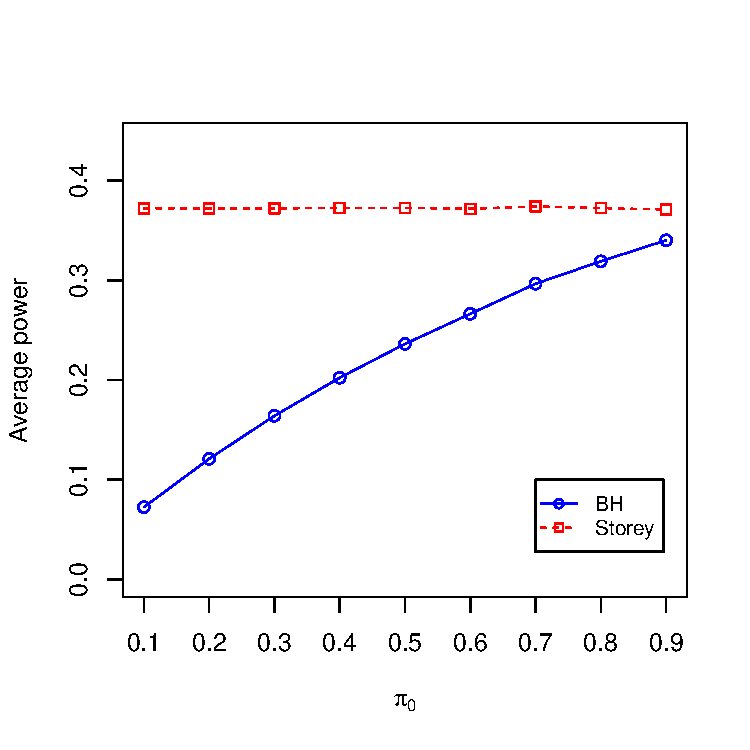
\includegraphics[width=0.5\textwidth]{../data/power.pdf}
	\caption{Average detection power comparison of BH procedure and direct approach.}
	\label{fig: power}	
\end{figure}

\section{Using Storey's estimator in Benjamini-Hochberg procedure} \label{sec: 2nd}

When using Storey's estimate $\widehat{\pi}_{0}$ of the proportion of true null hypotheses and $\widehat{\pi}_{0} \cdot m$ instead of $m$ in Benjamini-Hochberg procedure, the detection power of this improved Benjamini-Hochberg procedure is almost identical to Storey's direct approach. Even more, we can show that it is always greater or equal to detection power of Storey's direct approach.

\begin{proposition}
When using Storey's estimate $\widehat{\pi}_{0}$ in Benjamini-Hochberg procedure the detection power of Benjamini-Hochberg procedure is always greater or equal to detection power of Storey's direct approach.
\end{proposition}

\begin{proof}
Let $p_{1}, ..., p_{m}$ be observed ordered $p$-values and let's say that by using direct approach, we reject $l$ hypotheses corresponding to the first $l$ ordered observed $p$-values, so:
\begin{equation}
	l = \max \lbrace k : p_{(k)} \leq \gamma \rbrace.
\end{equation}
We then use Storey's method to estimate proportion $\widehat{\pi}_{0}$ of true null hypotheses and from this estimate of false discovery rate: $\widehat{\text{FDR}}_{\text{ST}}$. We then use BH procedure with control at level $\widehat{\text{FDR}}_{\text{ST}}$ and $\widehat{\pi}_{0} \cdot m$ instead of $m$ and calculate:
\begin{align}
	\hat{k} 
	&=\max \lbrace k : p_{(k)} \leq \frac{k}{\widehat{\pi}_{0} \cdot m} \cdot \widehat{\text{FDR}}_{\text{ST}} \rbrace \\
	&=\max \lbrace k : p_{(k)} \leq \frac{k}{\widehat{\pi}_{0} \cdot m} \cdot \frac{\widehat{\pi}_{0} \cdot \gamma}{l / m} \rbrace \\
	&=\max \lbrace k : p_{(k)} \leq \frac{k \cdot \gamma}{l} \rbrace.	
\end{align}
and because $p_{(l)} \leq \gamma$ it follows that:
\begin{equation}
	\hat{k} \geq l.
\end{equation}
So the set of hypotheses rejected by direct approach are contained in the set of hypotheses rejected by this improved BH procedure. 
\end{proof}

For this simulation we use the same setup as in the first but in BH procedure we use Storey's estimate $\widehat{\pi}_{0}$ of the proportion of true null hypotheses and $\widehat{\pi}_{0} \cdot m$ instead of $m$. From summary of the results in Table~\ref{tab: power_pi0_BH} and from Figure~\ref{fig: power_pi0_BH} we see that estimated average detection power of BH procedure is always greater than estimated average power of direct approach using Storey's estimators:
\begin{equation}
	\text{Power}_{\text{BH}} \geq \text{Power}_{\text{ST}}.
\end{equation}

\begin{table}[H]
	\centering	
	\begin{tabular}{cccccccc}
		$\pi_{0}$ & FDR$_{\text{ST}}$ & FDR$_{\text{BH}}$ & Power$_{\text{ST}}$ & Power$_{\text{BH}}$ & $\text{E} (\widehat{\text{FDR}}_{\text{ST}} )$ & $\text{E}(\widehat{\pi_{0}})$ & $\text{E}(\widehat{\gamma}_{\text{BH}})$ \\ 
		\hline
		0.1 & 0.003 & 0.003 & 0.372 & 0.373 & 0.004 & 0.141 & 0.0100 \\ 
		0.2 & 0.007 & 0.007 & 0.372 & 0.373 & 0.008 & 0.237 & 0.0100 \\ 
		0.3 & 0.011 & 0.011 & 0.372 & 0.373 & 0.013 & 0.332 & 0.0100 \\ 
		0.4 & 0.018 & 0.018 & 0.373 & 0.374 & 0.019 & 0.428 & 0.0100 \\ 
		0.5 & 0.026 & 0.026 & 0.373 & 0.374 & 0.027 & 0.523 & 0.0100 \\ 
		0.6 & 0.039 & 0.039 & 0.372 & 0.373 & 0.040 & 0.619 & 0.0100 \\ 
		0.7 & 0.057 & 0.058 & 0.374 & 0.376 & 0.060 & 0.713 & 0.0100 \\ 
		0.8 & 0.098 & 0.099 & 0.372 & 0.375 & 0.099 & 0.808 & 0.0100 \\ 
		0.9 & 0.193 & 0.197 & 0.371 & 0.377 & 0.200 & 0.906 & 0.0100 \\ 
		\hline
	\end{tabular}
	\caption{Average detection power comparison of BH procedure using $\widehat{\pi}_{0} \cdot m$ instead of $m$ and direct approach.}
	\label{tab: power_pi0_BH}	
\end{table}


\begin{figure}[H]
	\centering
	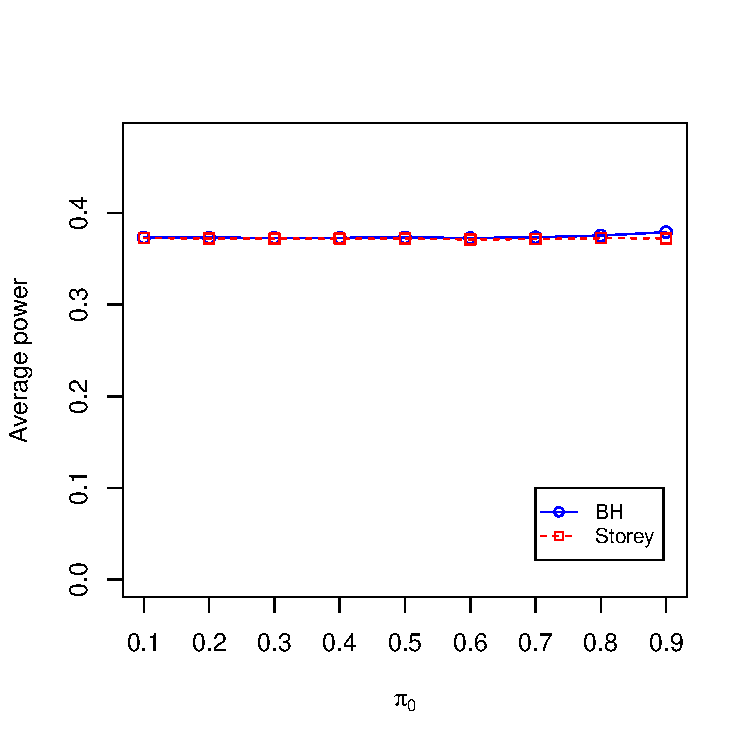
\includegraphics[width=0.5\textwidth]{../data/power_pi0_BH.pdf}
	\caption{Average detection power comparison of BH procedure using $\widehat{\pi}_{0} \cdot m$ instead of $m$ and direct approach.}
	\label{fig: power_pi0_BH}	
\end{figure}


\section{Properties of the Storey's estimator} \label{sec: properties}

In the previous two sections we showed that the estimator of $\pi_{0}$ plays a key role in detection power and in the estimation of error measure (p)FDR in the case of direct approach or equivalently in the level of control of FDR in the case of improved BH procedure when using estimator of $\pi_{0}$. Here we inspect some properties of this estimator.

Storey's estimator of the proportion of null hypotheses $\pi_{0}$ is:
\begin{equation}
\widehat{\pi_{0}}(\lambda) = \frac{W(\lambda)}{m \cdot (1-\lambda)},
\end{equation}
where $W(\lambda) = \# \lbrace p_{i} > \lambda \rbrace$ is the number of p-values greater than some value of parameter $\lambda$.

\begin{proposition}
	For any fixed value of $\lambda$ Storey's estimator $\widehat{\pi}_{0}$ at most overestimates $\pi_{0}$ in expectation:
	\begin{equation}
		\text{E}(\widehat{\pi}_{0}) \geq \pi_{0}.
	\end{equation}
\end{proposition}
\begin{proof}
	Let $U(\lambda) = \# \lbrace \text{null } p_{i} > \lambda \rbrace$ be the number of $p$-values from in fact true null hypotheses which exceeds $\lambda$ and $T(\lambda) = \# \lbrace \text{alternative } p_{j} > \lambda \rbrace$ corresponding number for the in fact false null hypotheses. Then $W(\lambda) = U(\lambda) + T(\lambda)$. If there are $m_{0}$ in fact true null hypotheses, then:
	\begin{equation}
		U \sim \text{Binomial}(m_{0}, 1 - \lambda)
	\end{equation}
	because $\text{Pr}(P \geq \lambda \mid H_{0}) = 1 - \lambda$ and
	\begin{equation}
		T \sim \text{Binomial}\left( m - m_{0}, \text{Pr}(P > \lambda \mid H_{1}) \right).
	\end{equation}
	Putting all this together we get:
	\begin{align}  %\tag{Bias}
		\text{E}(\widehat{\pi}_{0}) 
		&= \frac{ \text{E} \left[ U(\lambda)\right] + \text{E}\left[ T(\lambda) \right] }{m \cdot (1-\lambda)} \\
		&= \frac{m_{0} \cdot (1 - \lambda) + (m - m_{0}) \cdot \text{Pr}(P > \lambda \mid H_{1})}{m \cdot (1 - \lambda)}  \\
		&= \pi_{0} + (1 - \pi_{0}) \cdot \frac{\text{Pr}(P > \lambda \mid H_{1})}{1 - \lambda}  \label{eq: bias} \\
		&\geq \pi_{0}.
	\end{align}
\end{proof}

This inequality is guaranteed only in expectation and largely depends on a good choice of $\lambda$, as can be seen from the plot in Figure~\ref{fig: pi0_of_lambda}, where we choose the actual proportion of true null hypotheses to be 0.9: 
\begin{equation}
\pi_{0} = 0.9
\end{equation}
and vary the value of $\lambda$ in the range of $(0, 1)$. 

\begin{figure}[H]
	\centering
	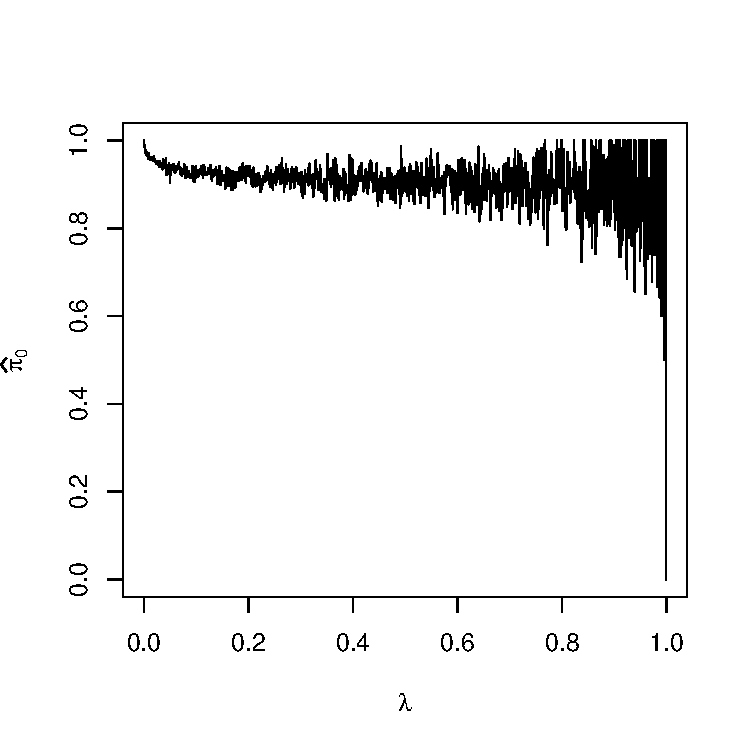
\includegraphics[width=0.5\textwidth]{../data/pi0_of_lambda.pdf}
	\caption{Storey's estimate $\widehat{\pi}_{0}$ of $\pi_{0} = 0.9$ depending on the value of the parameter $\lambda$.}
	\label{fig: pi0_of_lambda}	
\end{figure}

We introduce a new parameter $\mu_{1}$ which is the distance between the distributions associated with $H_{0}$ and $H_{1}$. We use the same simulation setup described in Section~\ref{sec: 1st} and simultaneously do $m = 1000$ one sided tests of null hypotheses, where the test statistics are in the form of observed $p$-values:
\begin{equation}
p_{i} = 1 - \Phi(z_{i}), % \text{Pr} \left[ N(0, 1) \geq z_{i} \right]
\end{equation}
where $z_{i}$ is the observed value of $Z_{i}$ under null hypothesis:
\begin{equation}
	Z_{i} \mid H_{0} \sim N(0, 1)
\end{equation} 

and under alternative hypothesis: 
\begin{equation}
	Z_{i} \mid H_{1} \sim N(\mu_{1}, 1).
\end{equation}

The estimates of $\text{E}(\widehat{\pi}_{0})$ over the range of $\pi_{0}$ depending on the values of $\mu_{1}$ and $\lambda$ are summarized in Table~\ref{tab: bias}. We see that the estimated upward bias increases, especially when $\pi_{0}$ is small, if we decrease the distance between the distributions $\mu_{1}$ from 2 to 1. This is true in general and follows from Equation~\ref{eq: bias} where we see the upward bias increases when probability of observing $p$-values corresponding to alternative hypothesis $H_{1}$ that are greater than $\lambda$, increases. This estimated upward bias is reduced if we increase $\lambda$, in this case from $0.5$ to $0.9$. This does not obviously follow from Equation~\ref{eq: bias} and it is hard to say anything in general (maybe in the limit when $\lambda \rightarrow 1$).

This same upward bias is present in estimates of FDR and pFDR, since estimate $\widehat{\pi}_{0}$ appears in the numerator of Storey's estimates of FDR and pFDR. Because of this, we only report estimated $\text{E}(\widehat{\pi}_{0})$ from this simulation.

\begin{table}[H]
	\centering	
	\begin{tabular}{ccccc}
		& \multicolumn{2}{c}{$\mu_{1} = 2$} & \multicolumn{2}{c}{$\mu_{1} = 1$} \\
		\cmidrule(lr){2-3} \cmidrule(lr){4-5}\\
		$\pi_{0}$ & $\lambda = 0.5$ & $\lambda = 0.9$ & $\lambda = 0.5$ & $\lambda = 0.9$  \\ 
		\hline
			0.1 & 0.141 & 0.105 & 0.384 & 0.202 \\ 
			0.2 & 0.236 & 0.206 & 0.454 & 0.290 \\ 
			0.3 & 0.332 & 0.306 & 0.522 & 0.378 \\ 
			0.4 & 0.428 & 0.402 & 0.590 & 0.468 \\ 
			0.5 & 0.523 & 0.504 & 0.658 & 0.559 \\ 
			0.6 & 0.618 & 0.601 & 0.727 & 0.643 \\ 
			0.7 & 0.715 & 0.700 & 0.795 & 0.735 \\ 
			0.8 & 0.808 & 0.798 & 0.864 & 0.827 \\ 
			0.9 & 0.906 & 0.900 & 0.930 & 0.908 \\ 
		\hline
	\end{tabular}
	\caption{Estimates $\text{E}(\widehat{\pi}_{0})$ depending on the values of parameters $\mu_{1}$ and $\lambda$.}
	\label{tab: bias}	
\end{table}

\section{Storey's bootstrap method for choosing the tuning parameter}
Storey proposed~\cite{Storey} a bootstrap procedure for choosing the optimal value $\lambda^{B}$ of parameter $\lambda$ which minimizes mean squared error of $\widehat{\pi}_{0}$. Using the same setup as before in Section~\ref{sec: 1st} we simultaneously do 1000 simulation of 1000 one sided tests and in each simulation use 1000 bootstrap samples (samples of $p$-values with replacements) to estimate the optimal value $\lambda^{B}$. Results are in Table~\ref{tab: bootstrap}. We see the estimated expected value of this bootstrap estimator $\text{E}(\widehat{\pi}^{B}_{0})$ is very close to the actual $\pi_{0}$ for all $\pi_{0}$ in the range $0.1, .., 0.9$. 

However in general the inequality:
\begin{equation}
	\text{E}(\widehat{\pi}_{0}) \geq \pi_{0}
\end{equation}
is no longer guaranteed for this estimator $\widehat{\pi}^{B}_{0} = \widehat{\pi}_{0}(\lambda^{B})$. The value of $\lambda$ is no longer fixed. In particular, choosing $\lambda$ that is associated with the smallest $\widehat{\pi}_{0}$ (or with smallest $\widehat{\text{pFDR}}$) will result in an underestimate of $\pi_{0}$ (and pFDR) as explained in~\cite{Black}. Storey and Tibshirani have proposed a cubic spline approach to estimating $\pi_{0}$ to alleviate some of the difficulties associated with this bootstrap procedure.

\begin{table}[H]
	\centering	
	\begin{tabular}{cc}
		$\pi_{0}$ &  $\text{E}(\widehat{\pi}^{B}_{0})$ \\ 
		\hline
		0.1 & 0.108 \\ 
		0.2 & 0.207 \\ 
		0.3 & 0.308 \\ 
		0.4 & 0.404 \\ 
		0.5 & 0.505 \\ 
		0.6 & 0.603 \\ 
		0.7 & 0.703 \\ 
		0.8 & 0.804 \\ 
		0.9 & 0.901 \\ 		
		\hline
	\end{tabular}
	\caption{Estimates $\text{E}(\widehat{\pi}^{B}_{0})$.}
	\label{tab: bootstrap}	
\end{table}


\section{Case of dependence} \label{sec: dependence}

To simulate dependence, we introduce a new parameter $\rho$, which is the degree of dependence between the distributions associated with $H_{0}$ and $H_{1}$. We simultaneously do $m = 1000$ one sided test of null hypotheses, where we test $H_{0i}: \mu = 0$ versus $H_{1i}: \mu > 0$ on the basis of $p$-values from simulated dependent random variables $Z'_{i}$, for $i = 1,...,m$ and:
\begin{equation}
Z'_{i} \sim Z_{i} + M,
\end{equation} 

where $M$ is random variable independent of $Z_{i}$ for each $i$ and normally distributed with parameters:
\begin{equation}
M \sim N(0, \rho) 
\end{equation} 
and $Z_{i}$ is, as in Section~\ref{sec: 1st}, distributed:
\[
Z_{i} \sim \begin{cases}
	N(0, 1) & \text{if $H_{0i}$ is in fact true,}\\
	N(2, 1) & \text{if $H_{1i}$ is in fact true.}
\end{cases}
\]
and proportion of in fact true null hypotheses $H_{0i}$ is $\pi_{0}$ out of all $m$ hypotheses.

$\newcommand{\E}{\mathrm{E}}$
$\newcommand{\Var}{\mathrm{Var}}$
$\newcommand{\Cov}{\mathrm{Cov}}$

From this we can calculate degree of dependence in terms of $\rho$:
\[
\mathrm{Cov} (Z_{i} + M, Z_{j} + M) = \begin{cases}
	\mathrm{Cov}(M, M) = \rho^2 & \text{if $i \neq j$,}\\
	\mathrm{Var}(Z_{i} + M) = 1 + \rho^2 & \text{if $i = j$}
\end{cases}
\]
and 
\[
\mathrm{Cor} (Z_{i} + M, Z_{j} + M) = \begin{cases}
	\frac{\rho^2}{1 + \rho^2} & \text{if $i \neq j$,}\\
	1 & \text{if $i = j$.}
\end{cases}
\]

On Figure~\ref{fig: dependence} we plotted upward bias of Storey's estimator $\widehat{\text{FDR}}_{\text{ST}}$ if we fix $\pi_{0} = 0.9$ and vary $\rho$ in range from 0 to 0.9. And in Table~\ref{tab: dependence} are summarized estimated Storey's estimators and estimated $\text{E}(\widehat{\gamma}_{\text{BH}})$ of BH procedure if we fix $\rho = 0.6$ and vary $\pi_{0}$. From Figure we see that degree of upward bias is very much influenced by the degree of dependence:
\begin{equation}
\text{E}(\widehat{\text{FDR}}_{\text{ST}}) >> \text{FDR}_{\text{ST}}, \qquad \text{for  } \rho > 0.
\end{equation}

For example in our simulation for $\rho = 0.6$ or:
\begin{equation}
	\mathrm{Cor}(Z'_{i}, Z'_{j}) = \frac{0.6^2}{1 + 0.6^2} \approx 0.26, \qquad i \neq j,
.\end{equation}
and $\pi_{0} = 0.9$, we have:
\begin{equation}
	\text{E}(\widehat{\text{FDR}}_{\text{ST}}) \approx 0.482 > 2 \cdot \text{FDR}_{\text{ST}} \approx 2 \cdot 0.228 = 0.456.
\end{equation}
So our simulation is showing that in this case Storey's estimate of FDR is more than 2 times larger than actual FDR on average when using direct approach.


\begin{figure}[H]
	\centering
	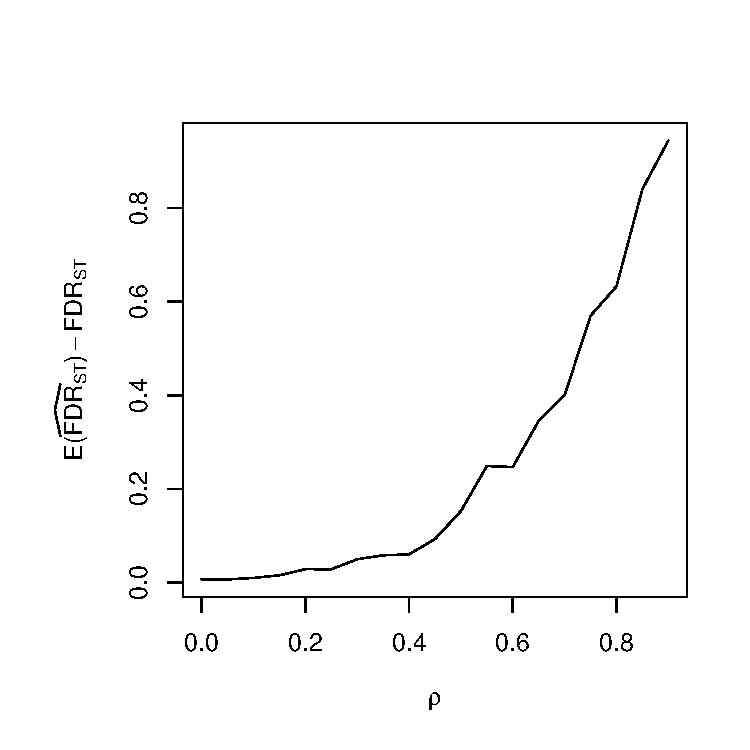
\includegraphics[width=0.5\textwidth]{../data/FDR_of_ro.pdf}
	\caption{Upward bias of Storey's $\widehat{\text{FDR}}_{\text{ST}}$ depending on the value of the parameter $\rho$, where $\pi_{0} = 0.9$.}
	\label{fig: dependence}	
\end{figure}


\begin{table}[H]
	\centering	
	\begin{tabular}{cccccccc}
		$\pi_{0}$ & FDR$_{\text{ST}}$ & FDR$_{\text{BH}}$ & Power$_{\text{ST}}$ & Power$_{\text{BH}}$ & $\text{E} (\widehat{\text{FDR}}_{\text{ST}} )$ & $\text{E}(\widehat{\pi_{0}})$ & $\text{E}(\widehat{\gamma}_{\text{BH}})$ \\ 
		  \hline
		0.1 & 0.004 & 0.001 & 0.387 & 0.093 & 0.014 & 0.178 & 0.0010 \\ 
		0.2 & 0.010 & 0.002 & 0.386 & 0.142 & 0.027 & 0.275 & 0.0030 \\ 
		0.3 & 0.017 & 0.006 & 0.394 & 0.185 & 0.036 & 0.358 & 0.0040 \\ 
		0.4 & 0.024 & 0.010 & 0.380 & 0.213 & 0.049 & 0.464 & 0.0050 \\ 
		0.5 & 0.038 & 0.018 & 0.396 & 0.257 & 0.079 & 0.536 & 0.0090 \\ 
		0.6 & 0.055 & 0.030 & 0.398 & 0.287 & 0.082 & 0.621 & 0.0100 \\ 
		0.7 & 0.077 & 0.052 & 0.387 & 0.316 & 0.136 & 0.730 & 0.0180 \\ 
		0.8 & 0.128 & 0.103 & 0.394 & 0.351 & 0.242 & 0.810 & 0.0300 \\ 
		0.9 & 0.228 & 0.256 & 0.390 & 0.428 & 0.482 & 0.908 & 0.0910 \\ 
		\hline
	\end{tabular}
	\caption{Upward bias of estimators in case of dependence $\rho = 0.6$.}
	\label{tab: dependence}	
\end{table}

\section{Conclusions}
We illustrate the duality between Storey's direct approach and Benjamini-Hochberg (BH) procedure when using Storey's estimate $\widehat{\pi}_{0}$ of proportion of null hypotheses $\pi_{0}$ in BH procedure. The performances of the two methods are almost identical in our simulations. This demonstrates that the estimator of $\pi_{0}$ plays a key role in multiple hypotheses testing. We show that Storey's estimator $\widehat{\pi}_{0}$ can be very upward biased when distance between distribution under null hypothesis $H_{0}$ and distribution under alternative hypotheses $H_{1}$ is small. In our simulations this upward bias of $\widehat{\pi}_{0}$ is reduced if we increase the value of $\lambda$ and especially by tuning the parameter $\lambda$ using Storey's bootstrap method. However this bootstrap method can result in underestimation of $\pi_{0}$. In case of dependence, we show by using simulation that dependence can lead to a very high overestimation of FDR.

\bibliographystyle{ieeetr}
\bibliography{main}

\end{document}